\documentclass[a4paper, 11pt]{article}
\usepackage{comment} 
\usepackage{fullpage} 
\usepackage[spanish]{babel} 
\selectlanguage{spanish}
\usepackage[utf8]{inputenc}
\usepackage{float} 
\usepackage{graphicx}
\usepackage{ marvosym }
\usepackage{amsthm}
\usepackage{amsmath}
\usepackage[sort&compress, numbers]{natbib}
\usepackage{amssymb}
\usepackage{hyperref}
\hypersetup{colorlinks=True, citecolor=blue}


\begin{document}
\begin{center}
\LARGE \bf Pr\'actica 1\\ Movimiento Browniano
\end{center}

\vspace{1cm} 
\noindent\textbf {Edson Edgardo Samaniego Pantoja} \hfill \textbf{Materia:} Simulación computacional 
\hfill \\
\textbf{Fecha} \today  
\vspace{1cm} 

\section{Introducción}
En esta primera pr\'actica se estudia el movimiento Browniano que refiere a una partícula que cambia su posición al azar de manera uniforme tomando su posición inicial el origen.

\section{Objetivo}
El objetivo principal de esta pr\'actica es observar los efectos por cada dimensión, para el tiempo de regreso al origen utilizando dimensiones de uno a cinco, se modifica el numero de pasos de la caminata como potencias de dos con exponente de cuatro a nueve y se hacen repeticiones de 30. Los resultados se graficaron con diagrama caja-bigote, aparte se incluye un cuadro indicando el mínimo, promedio y máximo del tiempo de regreso por cada dimensión junto con el porcentaje de caminatas que no regresaron. 

\section{Simulación}
Para la programación se explican ciertas partes importantes debido a que contiene l\'ineas repetitivas y extensas, el código completo puede ser consultado en github \cite{Edson}.De la mano es apoyada la programación con las practicas de Elisa Schaeffer en su github \cite{dra}
Se requieren librerías como \textit{random} para que la decisión sea al azar, \textit{matplotlib.pyplot} utilizada para la generación de diagramas caja-bigote, \textit{tabulate} para la obtención y visualización de datos y como extra por fines analíticos \textit{cv2} donde se utiliza la pausa en milisegundos para ver por pasos el programa.
\begin{verbatim}
from random import random, randint
import matplotlib.pyplot as plt
from tabulate import tabulate
import cv2 as cv2 #librería sólo por las pausas en los ciclos 
\end{verbatim}
Por medio de ciclos \textit{for} es como se hace el cambio tanto de dimensiones como de caminatas y las 30 replicas para obtener mayor conjunto de datos, dentro de las replicas se hace la decisión al azar tanto de la dimensión como el incremento a decremento unitario.
También se extrae la cantidad de regresos a cero, por replicas y por caminatas que se acumulan en una variable para m\'as adelante procesar y sacar el mínimo, máximo, promedio y porcentaje que no volvió nunca al origen. Utilizando paginas de apoyo \cite{Python2} para la programación y también desde la pagina oficial \cite{Python}.
\begin{verbatim}
for A in range(1, 6):
    dim = A
    
    for pot in range(4, 10):
        saltos = 2**pot
        rep= 30
        resultados = []
        nuevos = []# porque si no la lista se hace con None y no puedo extraer números
        datos=[],[],[],[],[],[]
        pos = [0] * dim
        
        for replica in range(rep):
            nunca = True
            for paso in range(saltos):
                cual = randint(0, dim -1)
                pos[cual] = pos[cual] + 1 if random()<0.5 else pos[cual] -1
                if all([p== 0 for p in pos]):
                    resultados.append(paso)
                    nuevos.append(paso)
                    nunca = False
                    break
\end{verbatim}
\begin{verbatim}
\end{verbatim}

\section{Resultados}
En este apartado se observan los diferentes resultados en las caminatas de 16, 32, 64, 128, 256 y 512 pasos, mostrados en gráficos caja-bigote.
Se observ\'o una tendencia a no volver a su origen conforme aumentan las dimensiones debido al n\'umero al azar, lo que lo vuelve menos probable que coincidan los orígenes. Solo en dimensiones 1 y 2 se logra ver que se mantienen los regresos moderados como se puede ver en la tablas \ref{tab1}, \ref{tab2} y las figuras \ref{cb16}, \ref{cb32}.

    \begin{table}[H]
        \caption{Caminatas de 16 pasos}
        \bigskip
        \label{tab1}
        \centering
        \begin{tabular}{|r|rrr|r|}
        \hline
        $dim$&$\min$&$\max$&$\mu$&$\%$\\
        \hline
        1 & 1 &  15 & 3.66 & 50 \\
        2 & 15 & 15 & 15 & 96.66\\
        3 & 0 &  0 & 0 & 100    \\
        4 & 0 &  0 & 0 & 100    \\
        5 & 0 &  0 & 0 & 100    \\
        \hline
        \end{tabular}
    \end{table}
    \begin{table}[H]
        \caption{Caminatas de 32 pasos}
        \bigskip
        \label{tab2}
        \centering
        \begin{tabular}{|r|rrr|r|}
        \hline
        $dim$&$\min$&$\max$&$\mu$&$\%$\\
        \hline
        1 & 1 & 9 & 2.64 & 43.33 \\
        2 & 1 & 17 & 3.72 & 63.33\\
        3 & 11 & 11 & 11 & 96.66    \\
        4 & 0 &  0 & 0 & 100    \\
        5 & 0 &  0 & 0 & 100    \\
        \hline
        \end{tabular}
    \end{table}
    \begin{table}[H]
        \caption{Caminatas de 64 pasos}
        \bigskip
        \label{tab3}
        \centering
        \begin{tabular}{|r|rrr|r|}
        \hline
        $dim$&$\min$&$\max$&$\mu$&$\%$\\
        \hline
        1 & 1 &  33 & 7.21 & 6.66 \\
        2 & 3 & 3 & 3 & 96.66 \\
        3 & 0 & 0 & 0 & 100    \\
        4 & 0 & 0 & 0 & 100    \\
        5 & 0 & 0 & 0 & 100    \\
        \hline
        \end{tabular}
    \end{table}
    \begin{table}[H]
        \caption{Caminatas de 128 pasos}
        \bigskip
        \label{tab4}
        \centering
        \begin{tabular}{|r|rrr|r|}
        \hline
        $dim$&$\min$&$\max$&$\mu$&$\%$\\
        \hline
        1 & 1 & 33 & 4.62 & 23.33 \\
        2 & 0 & 0 & 0 & 100\\
        3 & 5 & 5 & 5 & 96.66    \\
        4 & 0 & 0 & 0 & 100    \\
        5 & 0 & 0 & 0 & 100    \\
        \hline
        \end{tabular}
    \end{table}
    \begin{table}[H]
        \caption{Caminatas de 256 pasos}
        \bigskip
        \label{tab5}
        \centering
        \begin{tabular}{|r|rrr|r|}
        \hline
        $dim$&$\min$&$\max$&$\mu$&$\%$\\
        \hline
        1 & 1 & 213 & 15 & 0 \\
        2 & 3 & 149 & 76 & 93.33\\
        3 & 0 &  0 & 0 & 100    \\
        4 & 0 &  0 & 0 & 100    \\
        5 & 0 &  0 & 0 & 100    \\
        \hline
        \end{tabular}
    \end{table}
    \begin{table}[H]
        \caption{Caminatas de 512 pasos}
        \bigskip
        \label{tab6}
        \centering
        \begin{tabular}{|r|rrr|r|}
        \hline
        $dim$&$\min$&$\max$&$\mu$&$\%$\\
        \hline
        1 & 1 & 21 & 5.61 & 13.33 \\
        2 & 0 &  0 & 0 & 100\\
        3 & 0 &  0 & 0 & 100    \\
        4 & 0 &  0 & 0 & 100    \\
        5 & 0 &  0 & 0 & 100    \\
        \hline
        \end{tabular}
    \end{table}
    

A continuación se muestran los gráficos caja-bigote para ver la tendencia de los resultados de las tablas anteriores siendo ya más fácil de comprender como la dimensión 1 fue la más estable en regresos a origen ya que al ser un solo plano en el que puede cambiar de posición lo hace más probable y como conforme se aumentan las dimensiones ésta probabilidad de regresar se hace más lejana tanto que hay muchos casos que nunca vuelve.

\begin{figure}[H]
  \centering      
  \caption{caja-bigote 16 pasos}  
  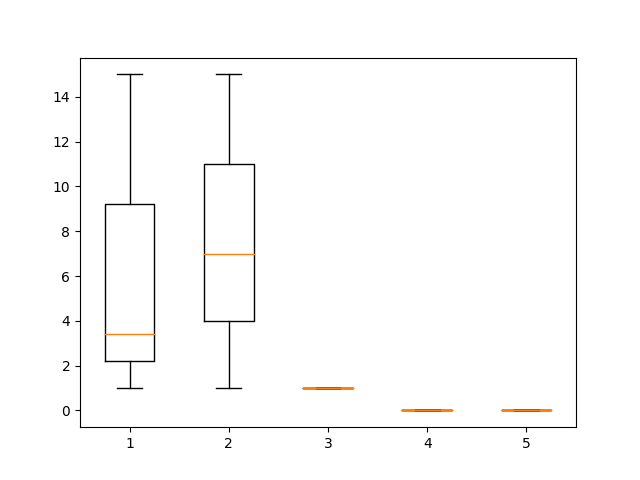
\includegraphics[scale=.7]{16_pasos.png}
  \label{cb16}
\end{figure}

\begin{figure}[H]
      \centering 
      \caption{caja-bigote 32 pasos}
      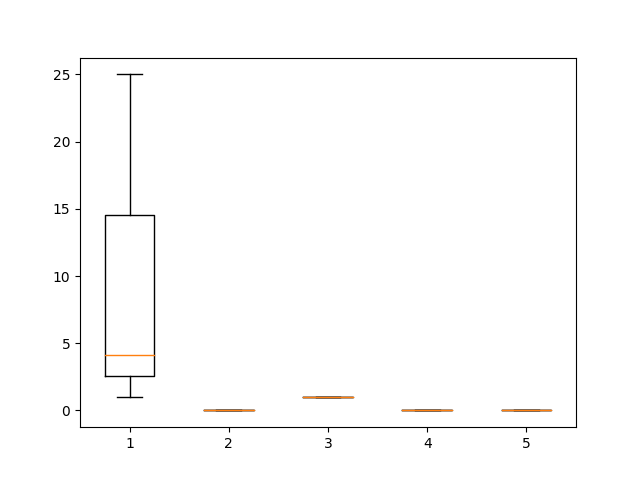
\includegraphics[scale=.7]{32_pasos.png} 
      \label{cb32}
\end{figure}

\begin{figure}[H]
      \centering
      \caption{caja-bigote 64 pasos} 
      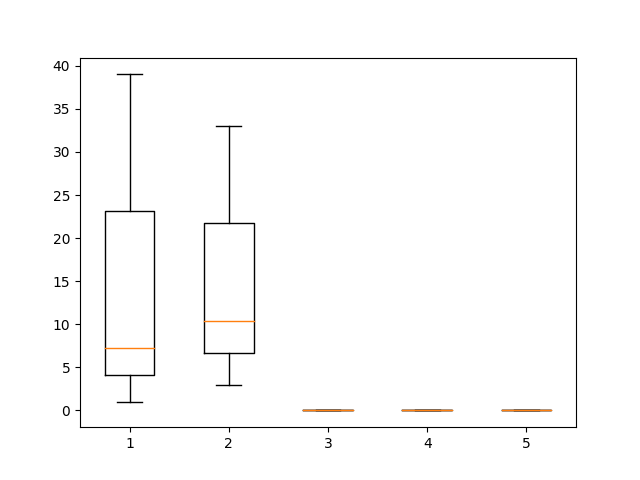
\includegraphics[scale=.7]{64_pasos.png}  
      \label{cb64}
\end{figure}

\begin{figure}[H]
      \centering
      \caption{caja-bigote 128 pasos}
      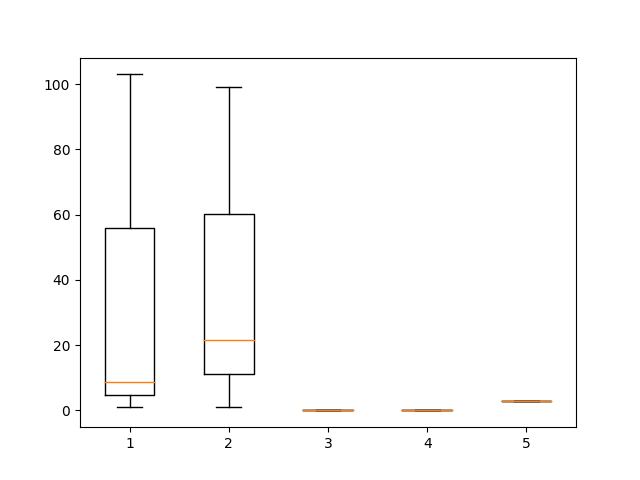
\includegraphics[scale=.7]{128_pasos.png} 
      \label{cb128}
\end{figure}

\begin{figure}[H]
      \centering                      % centra la imagen
      \caption{caja-bigote 256 pasos}
      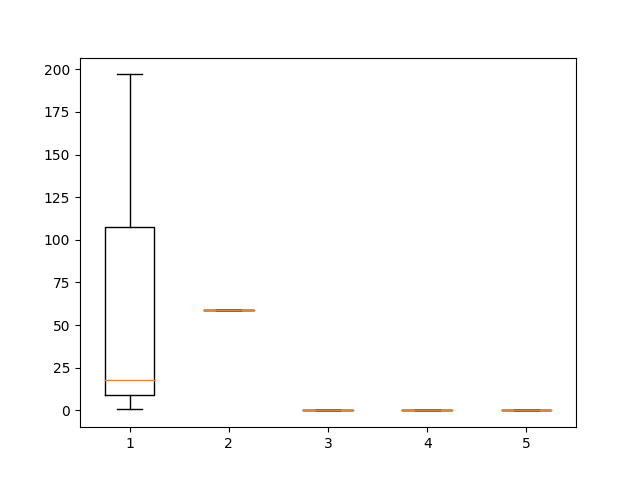
\includegraphics[scale=.7]{256_pasos.png}   
      \label{cb256}
\end{figure}

\begin{figure}[H]
      \centering 
      \caption{caja-bigote 512 pasos} 
      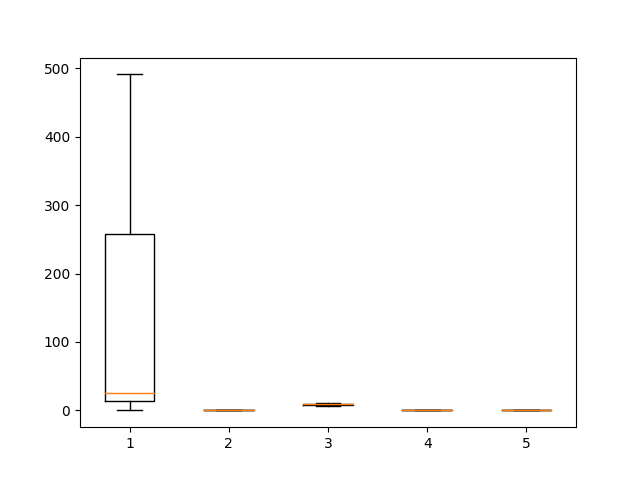
\includegraphics[scale=.7]{512_pasos.png}   
      \label{cb512}
\end{figure}

\bigskip
\bigskip
\bigskip
\bigskip
\bigskip
\bigskip
\bigskip
\bibliography{refe}
\bibliographystyle{plainnat}




\end{document}
